\begin{multicols}{3}
\begin{enumerate}
	\item \begin{minipage}[t]{\linewidth} Quel est l'angle alterne-interne à l'angle $\widehat{xDA}$ ?\\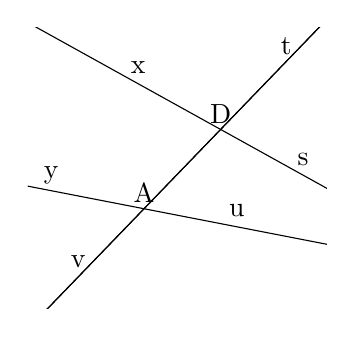
\begin{tikzpicture}[baseline,scale = 0.4]

    \tikzset{
      point/.style={
        thick,
        draw,
        cross out,
        inner sep=0pt,
        minimum width=5pt,
        minimum height=5pt,
      },
    }
    \clip (-4.736869106031488,-4.250328516779962) rectangle (4.7631758623361815,4.6700065683925605);
    	\draw[color={black}] (-42.34166861605179,25.679160612994153)--(45.99492180502718,-23.286611031885883);
	\draw[color={black}] (-33.343601782031854,-34.52831041625525)--(36.816893634326846,38.12500941794851);
	\draw[color={black}] (-50.123346728071695,8.461440068319265)--(49.02099880014237,-10.810268464711761);
	\draw[color={black}] (-35.77490607863836,-37.04599971744053)--(34.38558933772037,35.60732011676323);
	\draw [color={black}] (4.01,0.48) node[anchor = center,scale=1, rotate = 0] {s};
	\draw [color={black}] (-1.23,3.39) node[anchor = center,scale=1, rotate = 0] {x};
	\draw [color={black}] (3.47,4.1) node[anchor = center,scale=1, rotate = 0] {t};
	\draw [color={black}] (1.9,-1.15) node[anchor = center,scale=1, rotate = 0] {u};
	\draw [color={black}] (-3.99,-0.01) node[anchor = center,scale=1, rotate = 0] {y};
	\draw [color={black}] (-3.13,-2.74) node[anchor = center,scale=1, rotate = 0] {v};
	\draw [color={black}] (1.39,1.94) node[anchor = center,scale=1, rotate = 0] {D};
	\draw [color={black}] (-1.04,-0.58) node[anchor = center,scale=1, rotate = 0] {A};

\end{tikzpicture}\\ \end{minipage}
	\item \begin{minipage}[t]{\linewidth} Quel est l'angle alterne-interne à l'angle $\widehat{ADv}$ ?\\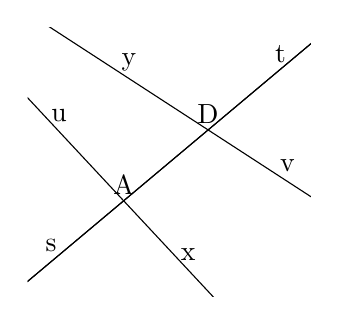
\begin{tikzpicture}[baseline,scale = 0.4]

    \tikzset{
      point/.style={
        thick,
        draw,
        cross out,
        inner sep=0pt,
        minimum width=5pt,
        minimum height=5pt,
      },
    }
    \clip (-4.197199994035402,-4.011010571846983) rectangle (4.798100590074228,4.532404376690253);
    	\draw[color={black}] (-40.40143951103323,28.51752697012443)--(44.30428785145457,-26.491015566393298);
	\draw[color={black}] (-36.770133269710925,-30.853805264953884)--(40.60035548530582,34.06774331338658);
	\draw[color={black}] (-35.24898466780339,35.603503666428715)--(33.632849698508956,-38.26322019710751);
	\draw[color={black}] (-39.45128882062737,-33.103561898856775)--(37.91919993438942,31.817986679483695);
	\draw [color={black}] (4.05,0.15) node[anchor = center,scale=1, rotate = 0] {v};
	\draw [color={black}] (-0.98,3.42) node[anchor = center,scale=1, rotate = 0] {y};
	\draw [color={black}] (3.83,3.71) node[anchor = center,scale=1, rotate = 0] {t};
	\draw [color={black}] (0.9,-2.66) node[anchor = center,scale=1, rotate = 0] {x};
	\draw [color={black}] (-3.2,1.73) node[anchor = center,scale=1, rotate = 0] {u};
	\draw [color={black}] (-3.45,-2.39) node[anchor = center,scale=1, rotate = 0] {s};
	\draw [color={black}] (1.53,1.79) node[anchor = center,scale=1, rotate = 0] {D};
	\draw [color={black}] (-1.15,-0.46) node[anchor = center,scale=1, rotate = 0] {A};

\end{tikzpicture}\\ \end{minipage}
	\item \begin{minipage}[t]{\linewidth} Quel est l'angle alterne-interne à l'angle $\widehat{BEy}$ ?\\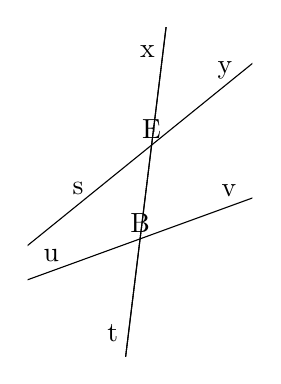
\begin{tikzpicture}[baseline,scale = 0.4]

    \tikzset{
      point/.style={
        thick,
        draw,
        cross out,
        inner sep=0pt,
        minimum width=5pt,
        minimum height=5pt,
      },
    }
    \clip (-3.751881877465446,-5.216457682385949) rectangle (3.3862738472500045,5.216457682385949);
    	\draw[color={black}] (-38.67449405774082,-29.977200325029884)--(39.81724804941324,33.584159171003684);
	\draw[color={black}] (-5.910663155149652,-48.13848835460412)--(6.3981405287702415,52.108672961169404);
	\draw[color={black}] (-47.16743505440314,-18.58982639374542)--(47.74151964497361,15.954208082147119);
	\draw[color={black}] (-6.276271185365095,-51.11612680952808)--(6.032532498554802,49.13103450624544);
	\draw [color={black}] (2.51,3.88) node[anchor = center,scale=1, rotate = 0] {y};
	\draw [color={black}] (-2.15,0.1) node[anchor = center,scale=1, rotate = 0] {s};
	\draw [color={black}] (0.05,4.47) node[anchor = center,scale=1, rotate = 0] {x};
	\draw [color={black}] (2.64,0.04) node[anchor = center,scale=1, rotate = 0] {v};
	\draw [color={black}] (-3,-2.01) node[anchor = center,scale=1, rotate = 0] {u};
	\draw [color={black}] (-1.05,-4.47) node[anchor = center,scale=1, rotate = 0] {t};
	\draw [color={black}] (0.18,1.99) node[anchor = center,scale=1, rotate = 0] {E};
	\draw [color={black}] (-0.18,-0.99) node[anchor = center,scale=1, rotate = 0] {B};

\end{tikzpicture}\\ \end{minipage}
	\item \begin{minipage}[t]{\linewidth} Quel est l'angle correspondant à l'angle $\widehat{uAt}$ ?\\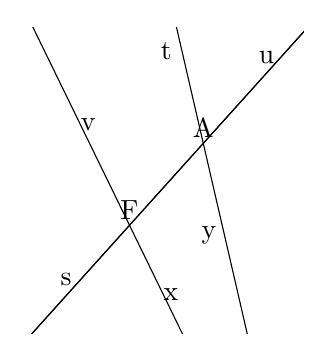
\begin{tikzpicture}[baseline,scale = 0.4]

    \tikzset{
      point/.style={
        thick,
        draw,
        cross out,
        inner sep=0pt,
        minimum width=5pt,
        minimum height=5pt,
      },
    }
    \clip (-4.571716929578387,-4.932671789852289) rectangle (4.199546898181071,4.787827432571796);
    	\draw[color={black}] (-10.243856807654957,49.83322047747786)--(12.476199681075396,-48.57815606583091);
	\draw[color={black}] (-32.45283440840463,-36.04252403565362)--(35.129356833840056,39.015103337563204);
	\draw[color={black}] (-23.256818552171588,43.45341266400355)--(21.01866727352523,-47.32478601221229);
	\draw[color={black}] (-34.79479153066063,-38.643530924824496)--(32.78739971158406,36.414096448392314);
	\draw [color={black}] (1.18,-1.81) node[anchor = center,scale=1, rotate = 0] {y};
	\draw [color={black}] (-0.17,4.04) node[anchor = center,scale=1, rotate = 0] {t};
	\draw [color={black}] (3.01,3.84) node[anchor = center,scale=1, rotate = 0] {u};
	\draw [color={black}] (-0.02,-3.68) node[anchor = center,scale=1, rotate = 0] {x};
	\draw [color={black}] (-2.65,1.71) node[anchor = center,scale=1, rotate = 0] {v};
	\draw [color={black}] (-3.35,-3.22) node[anchor = center,scale=1, rotate = 0] {s};
	\draw [color={black}] (1,1.61) node[anchor = center,scale=1, rotate = 0] {A};
	\draw [color={black}] (-1.34,-0.99) node[anchor = center,scale=1, rotate = 0] {F};

\end{tikzpicture}\\ \end{minipage}
	\item \begin{minipage}[t]{\linewidth} Quel est l'angle correspondant à l'angle $\widehat{yFu}$ ?\\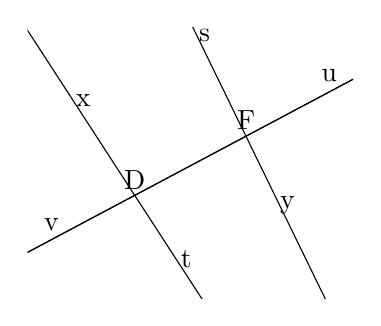
\begin{tikzpicture}[baseline,scale = 0.4]

    \tikzset{
      point/.style={
        thick,
        draw,
        cross out,
        inner sep=0pt,
        minimum width=5pt,
        minimum height=5pt,
      },
    }
    \clip (-5.164737964294635,-4.204954829408053) rectangle (5.164737964294635,4.385325264469283);
    	\draw[color={black}] (-20.152662153736017,45.878645440530136)--(24.122823671960802,-44.89955323568574);
	\draw[color={black}] (-42.381484457228495,-22.53463501372276)--(46.796222421523126,24.881992827652216);
	\draw[color={black}] (-28.997846936469212,40.99458527169941)--(26.010695600048535,-43.71114209078839);
	\draw[color={black}] (-45.9132748286642,-24.412521264866324)--(43.26443205008742,23.00410657650865);
	\draw [color={black}] (3.08,-1.26) node[anchor = center,scale=1, rotate = 0] {y};
	\draw [color={black}] (0.45,4.14) node[anchor = center,scale=1, rotate = 0] {s};
	\draw [color={black}] (4.41,2.85) node[anchor = center,scale=1, rotate = 0] {u};
	\draw [color={black}] (-0.13,-2.95) node[anchor = center,scale=1, rotate = 0] {t};
	\draw [color={black}] (-3.4,2.08) node[anchor = center,scale=1, rotate = 0] {x};
	\draw [color={black}] (-4.41,-1.85) node[anchor = center,scale=1, rotate = 0] {v};
	\draw [color={black}] (1.77,1.44) node[anchor = center,scale=1, rotate = 0] {F};
	\draw [color={black}] (-1.77,-0.44) node[anchor = center,scale=1, rotate = 0] {D};

\end{tikzpicture}\\ \end{minipage}
	\item \begin{minipage}[t]{\linewidth} Quel est l'angle alterne-interne à l'angle $\widehat{FCu}$ ?\\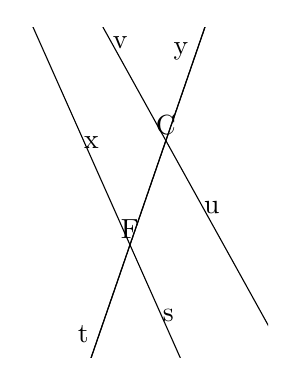
\begin{tikzpicture}[baseline,scale = 0.4]

    \tikzset{
      point/.style={
        thick,
        draw,
        cross out,
        inner sep=0pt,
        minimum width=5pt,
        minimum height=5pt,
      },
    }
    \clip (-3.7367342083748936,-5.004833590196926) rectangle (3.8946672956702804,5.4775928779965835);
    	\draw[color={black}] (-23.589344703402542,45.622022508168406)--(25.376426941477508,-42.71456791291054);
	\draw[color={black}] (-15.627271413943522,-45.38489162876719)--(17.255112186229304,50.11248450676377);
	\draw[color={black}] (-20.825184385475744,44.25899501873106)--(20.255216565180074,-48.009096203171616);
	\draw[color={black}] (-16.766759954543573,-48.694206643364815)--(16.11562364562926,46.80316949216618);
	\draw [color={black}] (2.11,-0.23) node[anchor = center,scale=1, rotate = 0] {u};
	\draw [color={black}] (-0.8,5.01) node[anchor = center,scale=1, rotate = 0] {v};
	\draw [color={black}] (1.13,4.73) node[anchor = center,scale=1, rotate = 0] {y};
	\draw [color={black}] (0.73,-3.66) node[anchor = center,scale=1, rotate = 0] {s};
	\draw [color={black}] (-1.71,1.82) node[anchor = center,scale=1, rotate = 0] {x};
	\draw [color={black}] (-1.97,-4.25) node[anchor = center,scale=1, rotate = 0] {t};
	\draw [color={black}] (0.65,2.39) node[anchor = center,scale=1, rotate = 0] {C};
	\draw [color={black}] (-0.49,-0.92) node[anchor = center,scale=1, rotate = 0] {F};

\end{tikzpicture}\\ \end{minipage}
	\item \begin{minipage}[t]{\linewidth} Quel est l'angle correspondant à l'angle $\widehat{uDx}$ ?\\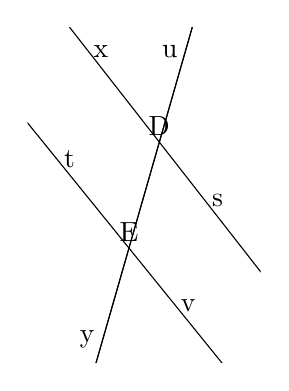
\begin{tikzpicture}[baseline,scale = 0.4]

    \tikzset{
      point/.style={
        thick,
        draw,
        cross out,
        inner sep=0pt,
        minimum width=5pt,
        minimum height=5pt,
      },
    }
    \clip (-3.6293280315809087,-5.075677631722435) rectangle (3.770040923495027,5.5563084796915945);
    	\draw[color={black}] (-30.231799054648906,41.323061072212724)--(31.95000995324256,-38.26602504206617);
	\draw[color={black}] (-13.230593079215955,-46.14056140503931)--(14.608779858300952,50.9468698847309);
	\draw[color={black}] (-31.879475586217374,37.41540552894106)--(31.681883909816214,-41.07633657821299);
	\draw[color={black}] (-14.195323824575457,-49.50497734082342)--(13.64404911294146,47.582453948946785);
	\draw [color={black}] (2.4,0.06) node[anchor = center,scale=1, rotate = 0] {s};
	\draw [color={black}] (-1.3,4.79) node[anchor = center,scale=1, rotate = 0] {x};
	\draw [color={black}] (0.88,4.81) node[anchor = center,scale=1, rotate = 0] {u};
	\draw [color={black}] (1.47,-3.27) node[anchor = center,scale=1, rotate = 0] {v};
	\draw [color={black}] (-2.3,1.39) node[anchor = center,scale=1, rotate = 0] {t};
	\draw [color={black}] (-1.74,-4.33) node[anchor = center,scale=1, rotate = 0] {y};
	\draw [color={black}] (0.55,2.42) node[anchor = center,scale=1, rotate = 0] {D};
	\draw [color={black}] (-0.41,-0.94) node[anchor = center,scale=1, rotate = 0] {E};

\end{tikzpicture}\\ \end{minipage}
	\item \begin{minipage}[t]{\linewidth} Quel est l'angle alterne-interne à l'angle $\widehat{ECv}$ ?\\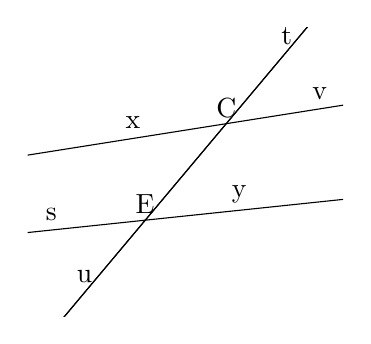
\begin{tikzpicture}[baseline,scale = 0.4]

    \tikzset{
      point/.style={
        thick,
        draw,
        cross out,
        inner sep=0pt,
        minimum width=5pt,
        minimum height=5pt,
      },
    }
    \clip (-5.019140905477899,-4.583099794098132) rectangle (4.998640241158492,4.58022221559489);
    	\draw[color={black}] (-48.098841810383796,-6.289634365773592)--(51.65768058972509,9.510246603289735);
	\draw[color={black}] (-30.853805264953884,-36.770133269710925)--(34.06774331338658,40.60035548530582);
	\draw[color={black}] (-51.011669987786746,-6.758512049620633)--(49.43504144440886,3.7988627404123747);
	\draw[color={black}] (-33.42495570370005,-39.83431104218686)--(31.49659287464043,37.536177712829925);
	\draw [color={black}] (4.25,2.5) node[anchor = center,scale=1, rotate = 0] {v};
	\draw [color={black}] (-1.68,1.56) node[anchor = center,scale=1, rotate = 0] {x};
	\draw [color={black}] (3.21,4.33) node[anchor = center,scale=1, rotate = 0] {t};
	\draw [color={black}] (1.7,-0.72) node[anchor = center,scale=1, rotate = 0] {y};
	\draw [color={black}] (-4.27,-1.35) node[anchor = center,scale=1, rotate = 0] {s};
	\draw [color={black}] (-3.21,-3.33) node[anchor = center,scale=1, rotate = 0] {u};
	\draw [color={black}] (1.29,2.03) node[anchor = center,scale=1, rotate = 0] {C};
	\draw [color={black}] (-1.29,-1.03) node[anchor = center,scale=1, rotate = 0] {E};

\end{tikzpicture}\\ \end{minipage}
	\item \begin{minipage}[t]{\linewidth} Quel est l'angle alterne-interne à l'angle $\widehat{DEu}$ ?\\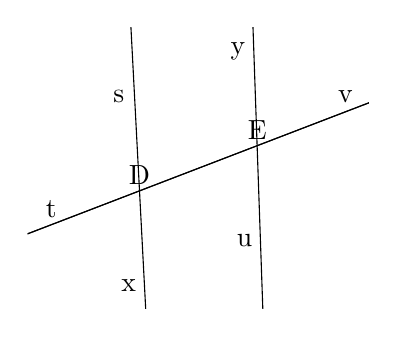
\begin{tikzpicture}[baseline,scale = 0.4]

    \tikzset{
      point/.style={
        thick,
        draw,
        cross out,
        inner sep=0pt,
        minimum width=5pt,
        minimum height=5pt,
      },
    }
    \clip (-5.417902132486009,-4.462624503354323) rectangle (5.417902132486009,4.464908380147888);
    	\draw[color={black}] (0.12218601786934635,50.68627725004538)--(3.647035184821962,-50.252196278883275);
	\draw[color={black}] (-44.81186047186567,-17.201661578174413)--(49.47976260435168,18.993501325900915);
	\draw[color={black}] (-4.483958665141602,49.21474083863809)--(0.8019729153957385,-51.646842171573866);
	\draw[color={black}] (-48.54618217785449,-18.635133376355615)--(45.74544089836289,17.560029527719713);
	\draw [color={black}] (1.47,-2.28) node[anchor = center,scale=1, rotate = 0] {u};
	\draw [color={black}] (1.26,3.71) node[anchor = center,scale=1, rotate = 0] {y};
	\draw [color={black}] (4.67,2.29) node[anchor = center,scale=1, rotate = 0] {v};
	\draw [color={black}] (-2.21,-3.71) node[anchor = center,scale=1, rotate = 0] {x};
	\draw [color={black}] (-2.52,2.28) node[anchor = center,scale=1, rotate = 0] {s};
	\draw [color={black}] (-4.67,-1.29) node[anchor = center,scale=1, rotate = 0] {t};
	\draw [color={black}] (1.87,1.22) node[anchor = center,scale=1, rotate = 0] {E};
	\draw [color={black}] (-1.87,-0.22) node[anchor = center,scale=1, rotate = 0] {D};

\end{tikzpicture}\\ \end{minipage}
\end{enumerate}
\end{multicols}
